\documentclass{article}

\newcommand{\authorname}{Austin Jetrin Maddison}
\newcommand{\course}{Discrete Simulation}
\newcommand{\courseid}{ICMA393}
\newcommand{\docname}{HW5}
\newcommand{\titletext}{\course: \docname}

%\usepackage{fontspec}	
\usepackage[no-math]{fontspec}	
\setmainfont{HelveticaNowText}
\newfontface\hh{HelveticaNowText-ExtraBold}
\newfontface\lt{HelveticaNowText-Light}      
\newfontface\xx{HelveticaNowText-ExtraLight} 
\newfontface\mm{HelveticaNowText Medium}

\newfontfamily{\displayfont}{HelveticaNowDisplay}
\newfontface\dslt{HelveticaNowDisplay-Light}
\newfontface\dsmm{HelveticaNowDisplay-Medium}
\newfontface\dsbd{HelveticaNowDisplay-Bold}

\newfontfamily{\microfont}{HelveticaNowMicro}
\newfontface\mclt{HelveticaNowMicro-Light}
\newfontface\mcmm{HelveticaNowMicro-Medium}
\newfontface\mcbd{HelveticaNowMicro-Bold}

\setmonofont{SFMono}

\usepackage[lining]{FiraSans}
\usepackage[fakebold]{firamath-otf}
\usepackage{unicode-math}
\setmathfont{FiraMath}
\renewcommand*\oldstylenums[1]{{\firaoldstyle #1}}

\usepackage{microtype}   % Improves text appearance with microtypography
\usepackage{amsmath}     % For better math support
\usepackage{graphicx}    % For including graphics
\usepackage{lipsum}      % For placeholder text
\usepackage{enumitem}
\usepackage{xcolor}
\usepackage{svg}
\usepackage{svg-extract}
\usepackage{caption}
\usepackage{float}
\usepackage{multicol}
\usepackage{booktabs}

\usepackage[a4paper, margin=0.8in, columnsep=20pt]{geometry}

\captionsetup{font=small}
\definecolor{gray}{rgb}{0.55, 0.55, 0.55}
\setlength{\columnsep}{20pt}  % Space between columns

% Headers and Footers
\usepackage{fancyhdr}
\pagestyle{fancy}
\fancyhf{}

% First Page
\fancypagestyle{plain}{
\fancyfoot[R]{\small \thepage} 
\fancyfoot[L]{} 
\fancyhead[L]{}
\fancyhead[R]{}
}

% Custom header
\fancyfoot[L]{\scriptsize \MakeUppercase{ \microfont \courseid~\course}}
\fancyhead[L]{\scriptsize \MakeUppercase{ \microfont \docname}}
\renewcommand{\headrulewidth}{0pt}

% Custom footer
%\fancyfoot[L]{\small Title, Date}
\fancyfoot[R]{\small \thepage}

% Line spacing
\usepackage{setspace}
\setstretch{1.15}  % Slightly more space between lines

%\setlength{\mathindent}{0pt} % This removes the indentation for equations

% Section formatting
\usepackage{titlesec}
\titleformat{\section}[block]{\raggedright \large\dsbd}{\thesection.}{1em}{}
\titleformat{\subsection}[block]{\normalsize \mm}{\thesubsection.}{1em}{}

% Bibliography style
\usepackage[numbers,sort&compress]{natbib} % For numbered citations

% Hyperlinks
\usepackage{hyperref}
\hypersetup{
    colorlinks=false,
    linkcolor=blue,
    citecolor=blue,
    urlcolor=blue,
    pdftitle={Research Paper Title},
    pdfauthor={Author's Name},
}

\usepackage{listings}
\lstset{
  language=Python,                     % Use Python language syntax
  basicstyle=\ttfamily\footnotesize,           % Use modern monospace font for code
  keywordstyle=\bfseries\color{black},   % Bold and blue keywords
  stringstyle=\color{black},              % Strings in red
  commentstyle=\color{gray},            % Comments in gray
  showstringspaces=false,               % Don't show spaces in strings
  breaklines=true,                      % Break long lines
  tabsize=4,                            % Set tab size to 4 spaces
}


\begin{document}
\fontsize{9.5}{11.5}\selectfont % Set font size to 12pt with a baseline of 14pt

% Title 
\title{
  \raggedright
  \Large \displayfont \strong{\courseid~\titletext} \\[5pt]  % Adjust spacing if needed
%  \raggedleft
  \small Mahidol University International College \\
  \small \authorname \\ 
  \small \today
}
\date{} 

%
%\twocolumn[{
%	\vspace*{-1cm}
%	\maketitle
%	\vspace*{-0.5cm}
%}]

\maketitle
%\raggedbottom
\section{Toilet Problem}

\noindent
I ran the simulation for $N=100000$ iterations, for the $Expo(Expo(Expo(Expo(371))))$.
\vspace{-2pt}
\begin{figure}[H]
	\centering
	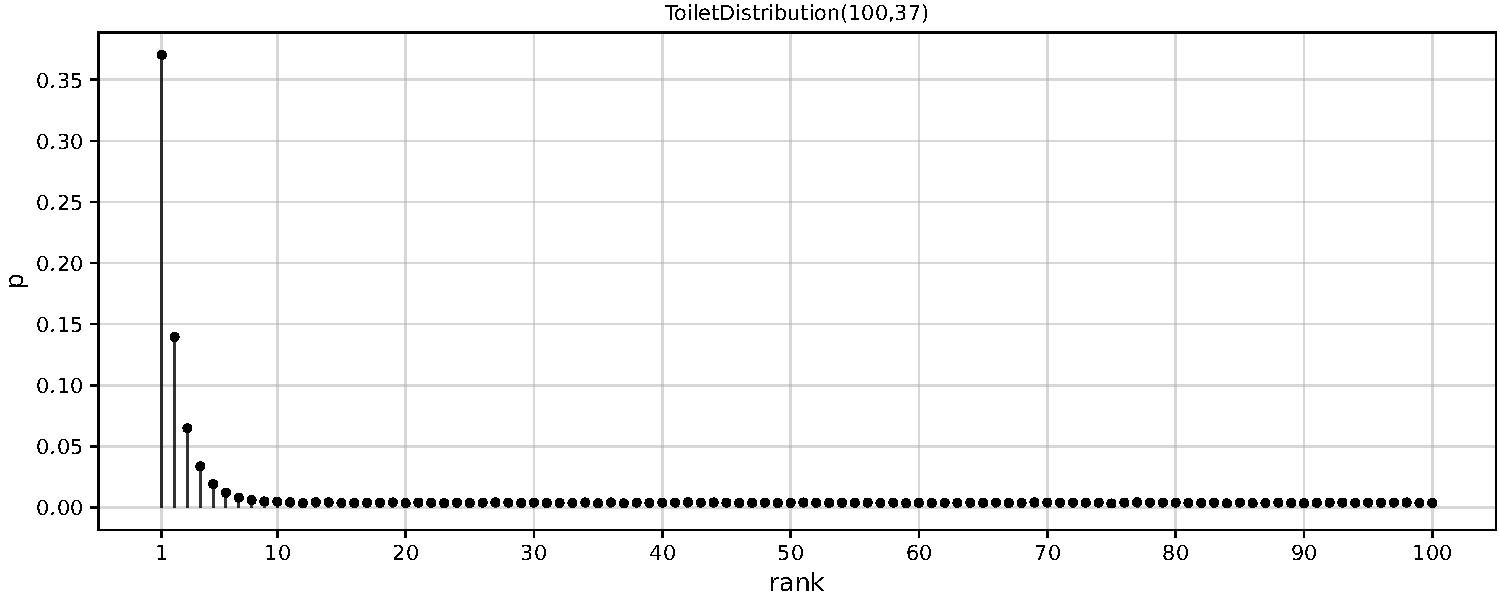
\includegraphics[width=1\linewidth]{../drawings/p1}
	\caption{The chained exponential distributions seems to follow Benford's law.}
	%	\label{fig:path1}
\end{figure}

\begin{lstlisting}
	[0.3704 , 0.13956, 0.06473, 0.03361, 0.01906, 0.01199, 0.00799,
	0.00589, 0.00481, 0.00463, 0.00414, 0.00349, 0.0042 , 0.00413,
	0.00349, 0.00359, 0.00371, 0.00374, 0.00399, 0.00341, 0.00391,
	0.00374, 0.00344, 0.00383, 0.00353, 0.00379, 0.004  , 0.0039 ,
	0.00359, 0.00386, 0.00363, 0.00363, 0.00366, 0.00399, 0.00333,
	0.00402, 0.00326, 0.00383, 0.00372, 0.00382, 0.00388, 0.00413,
	0.00392, 0.00399, 0.00383, 0.00351, 0.00367, 0.00385, 0.00364,
	0.00367, 0.00398, 0.00372, 0.00369, 0.00366, 0.00369, 0.00388,
	0.0035 , 0.00386, 0.0034 , 0.0036 , 0.00364, 0.00374, 0.00373,
	0.00374, 0.00364, 0.00397, 0.0035 , 0.0036 , 0.00401, 0.00397,
	0.0038 , 0.0039 , 0.00382, 0.00383, 0.00316, 0.00393, 0.00414,
	0.00389, 0.00394, 0.00379, 0.00371, 0.00363, 0.0038 , 0.00327,
	0.00395, 0.00341, 0.00344, 0.00393, 0.00356, 0.0034 , 0.00376,
	0.00389, 0.00396, 0.00369, 0.00382, 0.00366, 0.00396, 0.004  ,
	0.00367, 0.00364]
\end{lstlisting}


\section{Toilet Problem}


\section*{Source Code}
\href{https://github.com/AustinMaddison/discrete-simulation/tree/main/HW5/source}{https://github.com/AustinMaddison/discrete-simulation/tree/main/hw5/source}

% References
%\bibliographystyle{unsrt}
%\bibliography{references}

\end{document}
